\chapter{尺度关系与演示结果}
\section{无量纲比较}
采用$R/b=N^\nu$展示不同指数对应的尺寸变化，理想链取$\nu=1/2$；另一条曲线取$\nu=3/5$作为Flory近似的示意值，不能将其当作精确临界指数。
\begin{figure}[htbp]
  \centering
  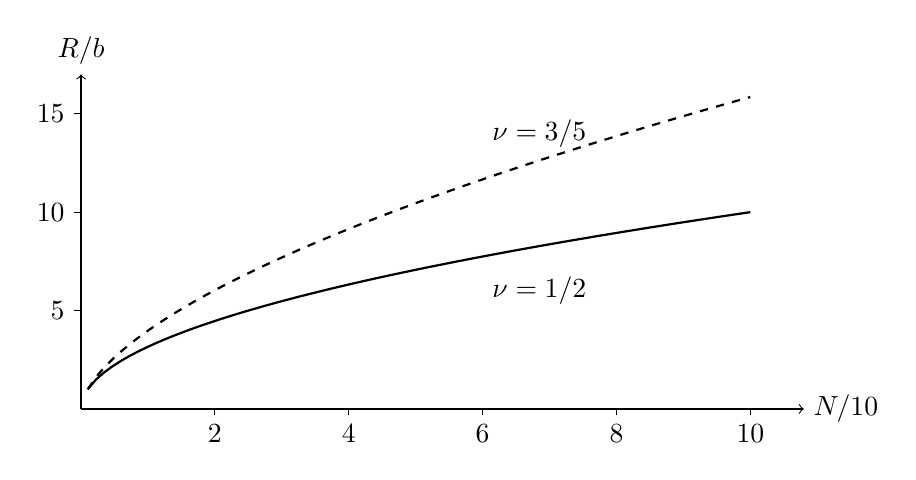
\begin{tikzpicture}[x=0.85cm,y=0.25cm]
    \draw[->] (0,0)--(10.8,0) node[right] {$N/10$};
    \draw[->] (0,0)--(0,17) node[above] {$R/b$};
    \draw[thick,domain=0.1:10,samples=80] plot (\x,{sqrt(10*\x)});
    \draw[thick,dashed,domain=0.1:10,samples=80] plot (\x,{(10*\x)^0.6});
    \node[right] at (6,6) {\scuSmallFont $\nu=1/2$};
    \node[right] at (6,14) {\scuSmallFont $\nu=3/5$};
    \foreach \x in {2,4,6,8,10} \draw (\x,0)--(\x,-0.3) node[below] {\scuSmallFont\x};
    \foreach \y in {5,10,15} \draw (0,\y)--(-0.1,\y) node[left] {\scuSmallFont\y};
  \end{tikzpicture}
  \caption{按指定幂律计算的链尺寸演示曲线}
  \label{fig:scaling}
\end{figure}

图\ref{fig:scaling}中的每一点都由公式直接生成。实测数据若呈现类似趋势，仍需检查测量范围、分子量分布和溶剂条件。
\begin{table}[htbp]
  \centering
  \caption{两种尺度描述的假设比较}
  \label{tab:models}
  \begin{tabular}{lll}
    \toprule
    模型 & 指数 & 主要前提\\
    \midrule
    理想链 & $1/2$ & 独立有效链段\\
    良溶剂Flory近似 & $3/5$ & 长链、排除体积作用\\
    \bottomrule
  \end{tabular}
\end{table}

\section{解释与验证}
表\ref{tab:models}中的前提属于解释的一部分。实验验证应比较多个链长区间，报告拟合区间变化带来的不确定性，并避免用同一组数据同时定义和验证结论。
